\section{Approximated Algorithms}
$APP(I)$, $I$ input, solution of approximation algorithm \\
$OPT(I)$, optimal solution \\
We want: $$APP(I) \stackrel{maximization \; problem}{\geq} \alpha OPT(I) + \beta \; \forall I$$
(for approximation problems we forget about decision problems since it doesn't make sense.) \\
If above holds then $APP(I)$ is called $\alpha-$approximation \\
Approximation schema: does not define a specific $\alpha$, but defines a time-optimality trade-off (spend more time $\Rightarrow$ get a better solution).

\subsection{Hamiltion Cycle Problem}
Is there a cycle which touches every vertex once?
\begin{center}
	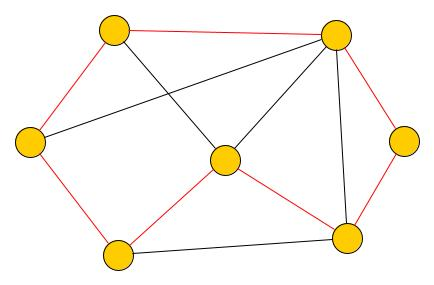
\includegraphics[scale=0.5]{img/graph27}
\end{center}
NP-Complete
\subsection{Eulerian Cycle Problem}
\begin{center}
	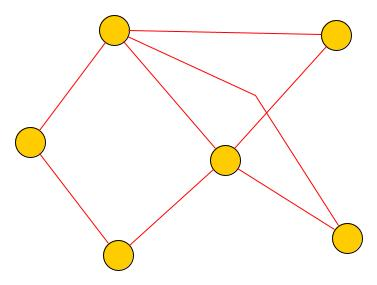
\includegraphics[scale=0.5]{img/graph28}
\end{center}
Cycle exists iff deg(v) is even $\forall v \in V$

($\Rightarrow$): easy, need to go through a vertex (in \& out) $\rightarrow \circ \rightarrow$ \\
($\Leftarrow$): suppose that every vertex has even degree $\Rightarrow$ eulerian cycle observation: 
\begin{center}
	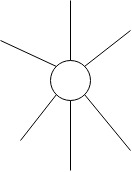
\includegraphics[scale=0.5]{img/vertex1}
\end{center}
take vertex and any two edges and split it into 
\begin{center}
	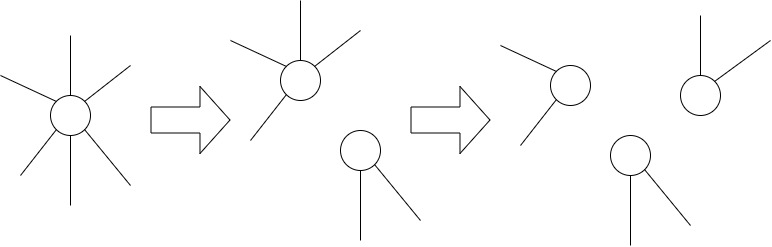
\includegraphics[scale=0.5]{img/vertex2}
\end{center}
$\Rightarrow$ Graph consists of cycles
\begin{center}
	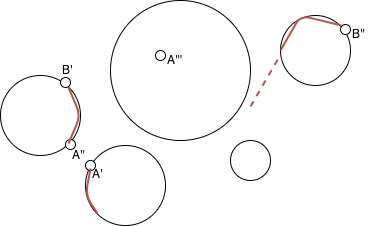
\includegraphics[scale=0.5]{img/vertex3}
\end{center}
construct cycle by arbitrary selecting a node and go along the cycle. If there is a vertex on the way which is a copy of a vertex, go to the next cycle. When a cycle is closed (vertex visited twice) go back. 
\subsection{TSP}
\begin{itemize}
	\item complete graph $K_n$
	\begin{center}
		$n=5:$ 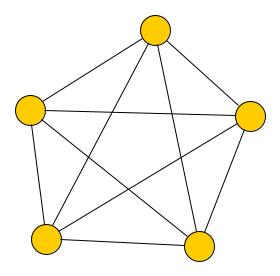
\includegraphics[scale=0.5]{img/graph29}
	\end{center}
	\item weights on the edges
	\item need one with minimum weight
	\item NP complete
\end{itemize}
\subsubsection{Reduction}
There is no construct that can approximate TSP 
$$\nexists \alpha : APP(I) \leq \alpha TSP(I) + \beta$$
"Inapproximability Result" \\
Suppose given a Graph $G$
\begin{center}
	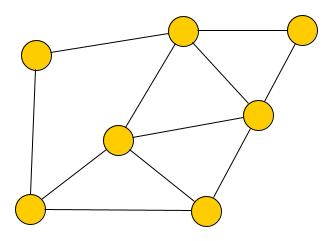
\includegraphics[scale=0.5]{img/graph30}
\end{center}
Specific graph $G \rightarrow K_n$ and weights
\begin{itemize}
	\item add missing edges with $n = |G|$ to get $K_n$
	\item weight of $e$ is, with $G = (V,E), K_n= (V',E')$,
		\begin{itemize}
			\item[1] if $e \in E$ $\forall e \in G \Rightarrow w(e) = 1$
			\item[$\alpha$] if $e \notin E$ $\forall e \notin G \Rightarrow n \cdot \alpha$
		\end{itemize}
	\item[$\Rightarrow$] starting at a problem/instance of the known problem 
	\item[$\Rightarrow$] construct an instance of the problem you want to lower bound
\end{itemize}
Assume we have a $\alpha-$approximation of TSP
\begin{itemize}
	\item[$\Rightarrow$] Hamiltonian Cycle could be solved in polynomial time
	\item[$\Rightarrow$] Hamiltonian Cycle $\in P \lightning$
\end{itemize}
Suppose $\exists$ Hamiltonian Cycle in $G$: $\Rightarrow \exists TSP$ with $cost = n \Rightarrow APP(I) \leq \alpha \cdot n$ \\
Suppose $\nexists$ Hamiltonian Cycle in $G$: $\Rightarrow \forall TSP$ has $cost > \alpha n\Rightarrow APP(I) > \alpha \cdot n$ \\
Metric $TSP$: weights satisfy the triangular inequality (also NP-complete!) \\
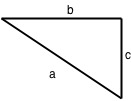
\includegraphics[scale=0.5]{img/tri} $a \leq b + c$ \\
2-approx \\
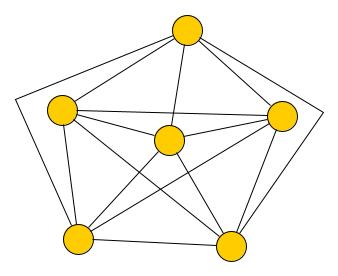
\includegraphics[scale=0.5]{img/graph31} $\stackrel{MST =: T}{\Rightarrow}$ 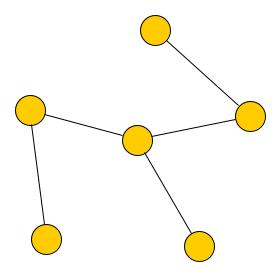
\includegraphics[scale=0.5]{img/graph32} \\
OPT ($=: \alpha$) \\
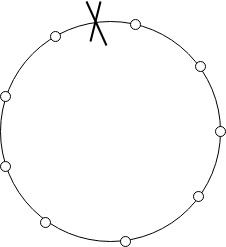
\includegraphics[scale=0.5]{img/st} by removing one edge wer get a spanning tree \\
$cost(T) \leq cost(spanning-path \alpha) < OPT$ \\
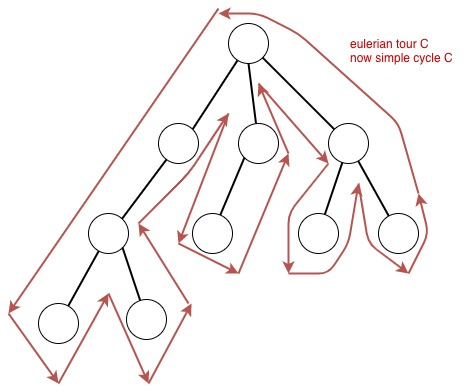
\includegraphics[scale=0.5]{img/cycle1} degree of $v$ gets doubled $\forall v \in V$ 
$$\Rightarrow cost(c) = 2 cost(T)$$
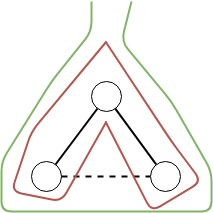
\includegraphics[scale=0.5]{img/cycle2} $C'=$ Hamiltonian Simple Cycle \\
Introduce shortcuts \\ $cost(C')=$? \\
replace the two edges by near one ... $\leq/+/$(triangle inequality!) \\
$cost(C') \leq cost(C)$
$$cost(C') \leq cost(C) = 2cost(T) \leq 2 \cdot OPT$$
Is the analysis tight? \\
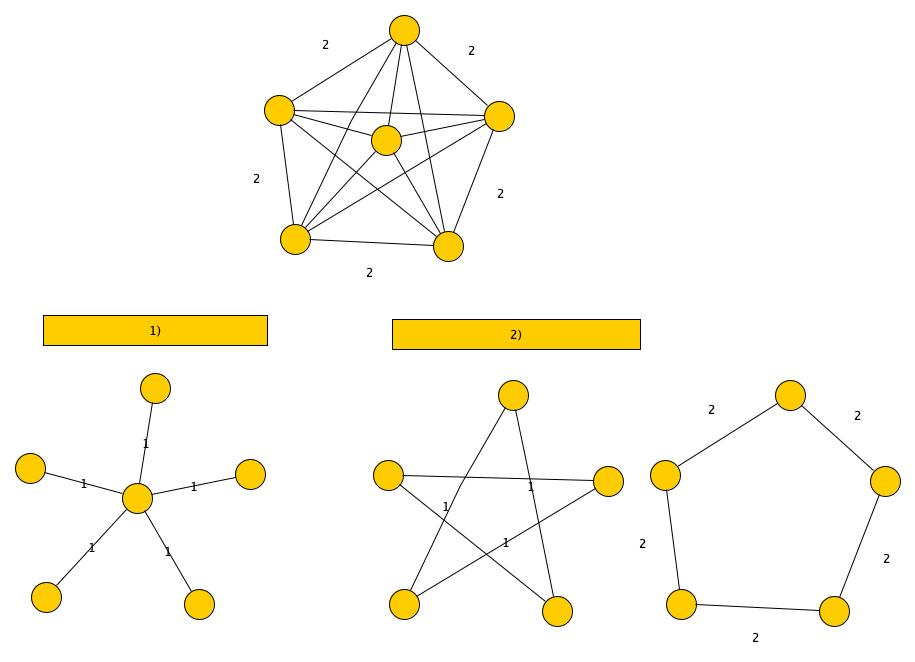
\includegraphics[scale=0.5]{img/graph33}
\subsection{MST}
either 1) or 2) \\
1): 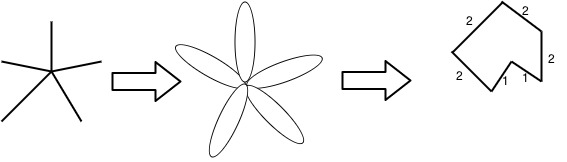
\includegraphics[scale=0.5]{img/mst1} $2n-2 \; cost$
\subsection{Christofides}
$$K_n \stackrel{MST}{\rightarrow}T \rightarrow \underbrace{V_0}_{\text{Set of ODD-DEG Vertice}} \stackrel{MIN-COST-PERF.-MATCH}{\longrightarrow} M \rightarrow T \cup M = C \stackrel{SHORTCUT}{\rightarrow} \underbrace{C'}_{hamiltonian \; cycle}$$
Where \\
$K_n$ like before\\
$T$: (E=even, O=odd) \\
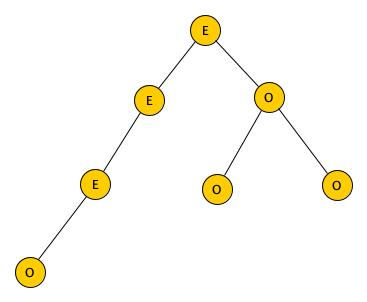
\includegraphics[scale=0.5]{img/graph19} \\
We can't have an odd number of vertices with an odd degree
$$\sum_{v \in T}\deg(v) = 2 |E|$$
$$\underbrace{\sum_{v \; ODD}\deg(v)}_{EVEN} + \underbrace{\sum_{v \; EVEN}\deg(v)}_{EVEN} = \underbrace{2 |E|}_{EVEN}$$
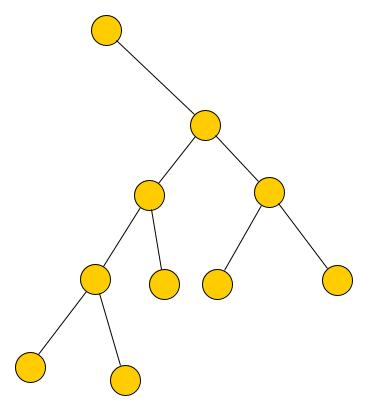
\includegraphics[scale=0.25]{img/graph20} All vertices have degree 3/1 ; 
 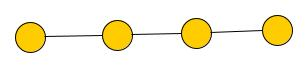
\includegraphics[scale=0.25]{img/graph21} All vertices have degree 2 except 2 \\
 $M$: \\
 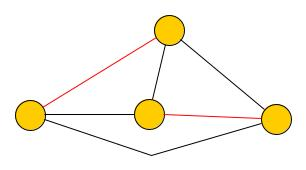
\includegraphics[scale=0.25]{img/graph22} Perfect Matching (red) (even number of vertices $\rightarrow \exists$ perfect matching) with Min-Cost \\
 $T \cup M$: \\
 1. red (even vertices?), 2. green (perfect match): 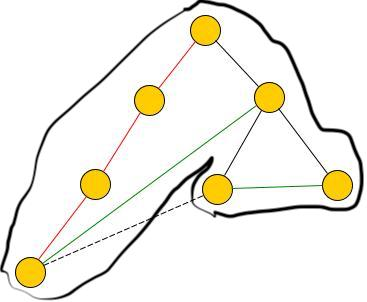
\includegraphics[scale=0.25]{img/graph23} \\
 \begin{align*}
 	cost(C') &\leq cost(C) & |\text{triangle inequality}\\
 	cost(C) &= cost(T) + cost(M) & |cost(T) < OPT,(*)  \\
 	cost(C_o^*) &\leq OPT & | (*1)	\\
 	(cost(M) \leq)cost(M^*) &\leq \frac{cost(C_0^*)}{2} & |cost(M) \leq \frac{OPT}{2} \\
 	cost(T) + cost(M) \leq \frac{3}{2}OPT
 \end{align*}
$$(*) C_0^* = \text{cycle derived from $C^*$ but only odd degree vertices}$$
$$(*1) \text{There are 2 perf. match. in } C_0^*, \text{take the minimal } M^*$$
We have everything we want, but we don't know whether we can do better or not. The best bound known is $\frac{3}{2}OPT$. Example that gets $\frac{3}{2}OPT$: (all edges without cost have cost 1, missing edges are very very expensive) \\
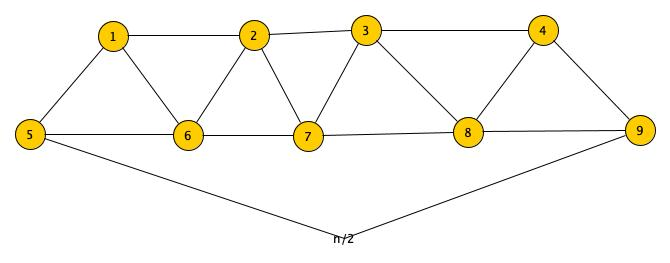
\includegraphics[scale=0.25]{img/graph24}
\\ OPT ($cost = n$): \\ 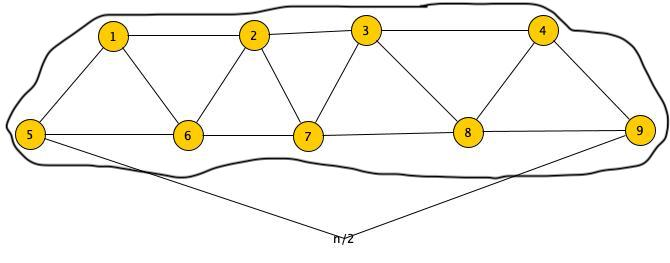
\includegraphics[scale=0.25]{img/graph25} \\
Consider the red $MST$ is found: \\ 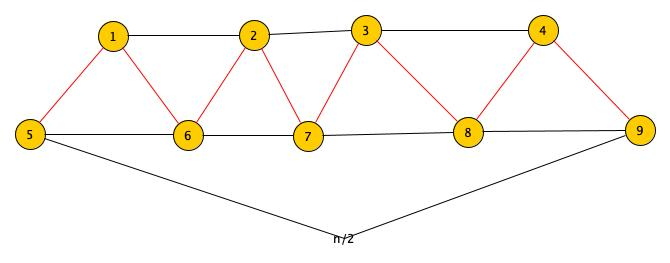
\includegraphics[scale=0.25]{img/graph26},\\ the perfect matching would include the n/2 edge that leads to a cycle. The cost is $n-1$ for the tree and $\frac{n}{2}$ for the edge. So: $\frac{3}{2}n$ \\
On the n/2 you can't put something greater than $\frac{n}{2}$ because of the triangle inequality. 
\subsection{PTAS: Polynomial Time Approximation Schema}
Schema: Not one approximation but an algorithm with a parameter. Balance between complexity and accuracy. \\
$\varepsilon > 0$ \\
Approx $\underbrace{(1 + \varepsilon)}_{Minimization}$ or $\underbrace{(1- \varepsilon)}_{Maximazation}$ \\
Time depends on $\frac{1}{\varepsilon}$ and $n$, possible approx.: $\underbrace{\mathcal{O}(n^{\frac{1}{\varepsilon}})}_{PTAS}$, much better: $\underbrace{\mathcal{O}(\frac{1}{\varepsilon}n)}_{F(ully)PTAS}$ 
\subsubsection{Knapsack}
\paragraph{Input}
$a_1,...,a_n$ items, each item has a size $s(a_i)$ and a profit $P(a_i)$. \\
Bag $B$ with a capacity $c(B)$
\paragraph{Output} Set of item $S$ that fits in the bag: 
$\sum_{a_i\in S}s(a_i) \leq c(B)$ and
maximize $\sum_{a_i \in S}P(a_i)$

simpler: $(\notin NP)$ raking functions of items \\
$A(i,P)$: smallest subset of the first $i$ items whose profit is equal to $P$ \\
Try to compote the first (specific value of a profit $\in \{1...\}$) $i$ items Knapsack, continue to $i+1 \in \{1...n\}$

Example: \\
\begin{tabular}{c|c|c}
& $s(a_i)$ & $P(a_i)$ \\ \hline 
$a_1$ & 3 & 20 \\
$a_2$ & 5 & 32 \\
$a_3$ & 4 & 40 \\
$a_4$ & 1 & 28 \\
$a_5$ & 2 & 20 \\
\end{tabular} \\
$A(5,100)$: \\
$a_2,a_3,a_4 \rightarrow P = 100, s = 10$ \\
$a_1,a_2,a_4,a_5 \rightarrow P = 100, s = 11$ \\
$A(5,99) = \infty$ \\
\begin{tabular}{cccccc|c|}
	& $i \rightarrow $ & 1 & 2 & 3 & ... & n \\
	& 1 & $\infty$ & $\infty$ & & & \\
	& 2 & $\infty$ & $\infty$ & & & \\
	& 3 & $\infty$ & $\infty$ & & & \\
	& ... & ... & ... & & & \\
	20 & ... & 3 & 3 & & & $\leq B$ \\
	& ... & ... & $\infty$ & & &  \\
	32 & ... & ... & 5 & & &  \\
	& ... & ... & $\infty$ & & &  \\
	52 & ... & ... &85 & & &  \\
	& ... & ... & $\infty$ & & &  \\
	& n & $\infty$ & ... & && \\
	& $\uparrow$ &&&&& $\uparrow$ \\
	& $P$ &&&&& \\
\end{tabular} \\
$$A(i,P) = \begin{cases}
s(a_i) + A(i-1,P-P(a_i)) & use \; i \\A(i-1,P) & don't \; use \; i
\end{cases}$$
stop at $A(n,n \cdot \underbrace{P_M}_{max \; profit \; of \; an \; item})$ $\rightarrow$ Solution $S$ cannot get better! \\
then read the table (last column) \\
complexity: $\#cells$, $\mathcal{O}(n\cdot n \cdot P_M) = \mathcal{O}(n^2 \cdot P_M)$ \\
$P_M$ is problem, because $P_M$ is a number $\Rightarrow$ represented in logarithmic number of bits $\Rightarrow$ input $\log$ $\Rightarrow$ output exonential ($\Rightarrow\in NP$) in terms of input. \\
$$ K = \frac{\varepsilon \cdot P_M}{n} \Rightarrow P^*(a_i) = \lfloor \frac{P(a_i)}{K} \rfloor $$
obtain complexity: $$\mathcal{O}(n^2 \cdot P_M^*) = \mathcal{O}(n^2 \cdot \lfloor \frac{P_M}{\underbrace{\varepsilon \cdot P_M}_{n}} \rfloor
) = \mathcal{O}(\frac{n}{\varepsilon})$$
$S^*$ set computed on the star instance \\
know: $S^* = OPT^*$ \\
compare to: $OPT = S_0$
$$\frac{P(a_i)}{K}-1 \leq P^*(a_i) \leq \frac{P(a_i)}{K} (da \lfloor\rfloor )$$
\begin{align*}
	&P(a_i) - K P^*(a_i) \leq K \forall i \\
	&\stackrel{\sum_{S_0}}{\Rightarrow} \underbrace{\sum_{a_i \in S_0}(P(a_i) - KP^*(a_i))}_{P(S_0) = KP^*(S_0) \leq K_n} \\
	& \leq K|S_0| \leq K_n \\
	P(S^*) &\leq KP^*(S^*) \geq K\underbrace{P^*(S_0)}_{\text{just some solution in $P^*$ and $S^* = OPT$}} \geq P(S_0) - K_n \geq OPT - K_n \\
	&= OPT - \varepsilon P_M \stackrel{P_M \leq OPT}{\geq} OPT - \varepsilon OPT \\
	&= (1 - \varepsilon) \cdot OPT
\end{align*}
\subsubsection{Bin Packing}
\paragraph{Input} $a_1,...,a_n$ items with sizes $s(a_1),...,s(a_n)$, $\forall i s(a_i) \leq 1$. No profits. We want to fit all items in a certain number of bins. We have maximal $n$ bins (every item one bin), but want minimal number of bins. Bin-size is 1.
\paragraph{Output} Configuration to fit $a_1,...,a_n$ in minimal number of bins. \\
to be continued ...
\subsubsection{2-Partition}
Strong related to Bin Packing (pack items in two bags). 
\paragraph{Input} $i_1,...,i_n$ Integers
\paragraph{Output} Partition of $i_1,...,i_n$ in two partitions $I_1,I_2$ with $$\sum_{i \in I_1}i = \sum_{i \in I_2}i$$

Reduction between these two problems 2-Partition $\leq$ Bin Packing: Positive instance $i_1,...i_n$ means they fit into 2 bins, else they don't. 

\paragraph{Approximation}
The approximation is $\frac{3}{2}$ (positive instance). There is no $\alpha \leq \frac{3}{2}$. \\
PTAS: $(1+\varepsilon) \rightarrow$ PTAS doesn't exist (inaproximability) $\Rightarrow$  APTAS

\subsection{APTAS}
Asymptotic PTAS. Look at large instances $\Rightarrow \frac{n+1}{n} \frac{n (1+\frac{1}{n})}{n} \rightarrow 1$ \\ 
$$ALG(I) \leq (1+ \varepsilon)OPT + C$$
Add a constant $C$ to handle extreme cases in small instances

\subsubsection{Bin Packing (continuation)}
Greedy approach
\begin{itemize}
	\item $a_1$ in $bin_1$
	\item $a_2$: does it fit in $bin_1$? yes: put it in $bin_1$, else in $bin_2$ (then $bin_1$ is closed)
	\item $a_3$: does it fit in the current? ...
\end{itemize}
$\Rightarrow$ try to fit it into the current bin, if it doesn't fit, got to the next bin. \\ \newline 
Optimal solution: all bins are completely full $\Rightarrow OPT \; bins \Rightarrow \sum i = OPT$ \\
There could be $bin$s that are nearly empty, because the next item doesn't fit in the bin, so the bin stays nearly empty (even if there were other items that fit in). \\
Connect $bin_1,bin_2$ and $bin_3,bin_4$,.... For each pair the sum is $>1$ and $\leq 2$. $\Rightarrow$ Approximation with factor 2. \\ 
\paragraph{APTAS} instance $I$: $1,3,3, 5, 6, 6, 8, 10, 12, 14$. Select $\varepsilon = 4$ \\ \newline 
$\underbrace{1,3,3}_{small (<4)} | \underbrace{5, 6, 6, 8, 10, 12, 14,16}_{large}$ \\ \newline 
$I_L = \underbrace{5,6,6}_{=\frac{|I_L|}{k}},\underbrace{8,10,12}_{=\frac{|I_L|}{k}},\underbrace{14,16}_{\leq\frac{|I_L|}{k}}$, bin capacity $c$, items $\geq \varepsilon \rightarrow  \frac{c}{\varepsilon}$ items maximal \\ \newline  
$I_L':6,6,6 | 12,12,12 | \times$ $$\Rightarrow ALG(I_L') \stackrel{brute-force}{=}OPT(I_L')$$ \\
Now: $ALG(I_L') \rightarrow ALG(I_L) \rightarrow ALG(I)$ and how does it change the relationship to $OPT(I_L), OPT(I)$ \\ \newline 
$ALG(I_L') \rightarrow ALG(I_L)$: Split $I_L'$ to the bins. Replace the Element by their real value (works because they just got greater in $I_L'$). The last group $\times$ just gets a bin for each item. $$ALG(I_L) \leq ALG(I_L') + \frac{|I_L|}{k}$$
$OPT(I_L) \rightarrow OPT(I_L')$ The last element in the first $I_L'$ group is smaller than the first in the next group in $I_L$. So every group in $I_L'$ can be mapped to the next group in $I_L$. The last group of $I_L$ remains . \\
We have an optimal solution for $I_L$ given. Cut the elements of the first group. replace group 2 elements of $I_L$  by group 1 elements of $I_L'$. In the example: replace in $OPT$-solution: $8,10,12$ by $6,6,6$. \\
\begin{center}
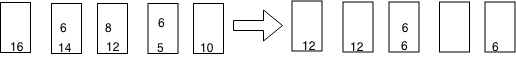
\includegraphics[scale=0.5]{img/bin-pack} 
\end{center}
$$OPT(I_L') \leq OPT(I_L)$$
$$ALG(I_L) \leq ALG(I_L') + \frac{|I_L|}{k} = OPT(I_L') + \frac{|I_L|}{k} \leq OPT(I_L) + \frac{|I_L|}{k}$$
Chosse $k = \frac{1}{\varepsilon^2}$. The following holds: $OPT(I_L) \geq \sum sizes \geq |I_L|\varepsilon$. So:
$$ OPT(I_L) + \frac{|I_L|}{k} = OPT(I_L) + |I_L|\varepsilon^2 \leq OPT(I_L) + OPT(I_L) \cdot \varepsilon  = (1+ \varepsilon) OPT(I_L)$$
$$\Rightarrow ALG(I_L) \leq (1+\varepsilon)OPT(I_L)$$
Now we want to go back to the initial instance. So we need to put the small item somewhere. For that use the greedy approach and just fill the gaps.
\begin{enumerate}
	\item All small elements fit in the gaps $\Rightarrow ALG(I) = ALG(I_L) \checkmark$, we are ok
	\item Otherwise: We need extra bin(s). If they don't fit create a new bin and try to fit them there. If this is full get a new one and so on. But there are still gaps in the bins before. There can't be any elements greater than $\varepsilon$ (they are filled by $1-\varepsilon$ if the capacity is 1).
	$$(ALG(I)-1) \cdot (1-\varepsilon) \leq \sum sizes \leq OPT(I)$$
	$$ALG(I) \leq \frac{OPT(I)}{1-\varepsilon}+1$$
	(The 1 (=$C$) defines the APTAS) \\
	for $\varepsilon \leq \frac{1}{2} \rightarrow 1 + 2 \varepsilon$
		$$ALG(I) \leq \frac{OPT(I)}{1-\varepsilon}+1 \leq (1+2\varepsilon)OPT(I) + 1$$
\end{enumerate}